\documentclass{article}

\usepackage{arxiv}

\usepackage[utf8]{inputenc} % allow utf-8 input
\usepackage[T1]{fontenc}    % use 8-bit T1 fonts
\usepackage{hyperref}       % hyperlinks
\usepackage{url}            % simple URL typesetting
\usepackage{booktabs}       % professional-quality tables
\usepackage{amsfonts}       % blackboard math symbols
\usepackage{nicefrac}       % compact symbols for 1/2, etc.
\usepackage{microtype}      % microtypography
\usepackage{lipsum}		% Can be removed after putting your text content
\usepackage{amssymb,amsmath}
\usepackage{listings}
\usepackage{graphicx}
\usepackage{subfig}
%\usepackage{apacite}

\title{Policy interventions for eradication of SARS-CoV-2 by mobile-phone contact-tracing}

%\date{September 9, 1985}	% Here you can change the date presented in the paper title
%\date{} 					% Or removing it

\author{
  Daniel Tang\\
  Leeds Institute for Data Analytics\thanks{This project has received funding from the European Research Council (ERC) under the European Union’s Horizon 2020 research and innovation programme (grant agreement No. 757455)}\\
  University of Leeds\\
  Leeds, UK\\
  \texttt{D.Tang@leeds.ac.uk} \\
  %% examples of more authors
  %% \AND
  %% Coauthor \\
  %% Affiliation \\
  %% Address \\
}

\begin{document}
\maketitle

\begin{abstract}
With the recent announcement\cite{applegoogle} that Apple and Google will introduce a contact-tracing API to iOS and Android, and later add contact tracing functionality directly to their OS's, it seems increasingly likely that contact tracing via a smart phone will form an important part of the effort to manage the COVID-19 pandemic and prevent resurgences of the disease after an initial outbreak.
 
However, contact-tracing models have shown \cite{Ferrettieabb6936}\cite{hellewellfeasibility} that there remains a high degree of uncertainty over whether contact tracing alone will be enough to control the virus. Here, we suggest complementary policies that could be used as part of a responsive policy to increase the effectiveness of smart phone contact tracing in the event that a resurgence looks imminent.
\end{abstract}

% keywords can be removed
\keywords{COVID-19, SARS-CoV-2}

\section{Introduction}

Contact-tracing models\cite{Ferrettieabb6936}\cite{hellewellfeasibility} have shown that contact-tracing using a mobile phone app has the potential to control and possibly even eradicate SARS-CoV-2. However, the results from these models, along with those from our own model, show that the uncertainty in $R0$ and in the amount of asymptomatic transmission (in the form of transmission from asymptomatic carriers and pre-symptomatic transmission) means that we cannot be certain that mobile-phone contact tracing alone will prevent a resurgence of the disease.

In previous publications, results have been shown in terms of the proportion of contacts traced. It is important to distinguish between the proportion of people using the app and the proportion of contacts traced. Current smart phone ownership among UK adults was 88\% as of 2019\cite{deloitte}. Ownership among teenagers is similar\cite{statistica}\footnote{younger children would have to be issued with bluetooth tracing devices in order to be traced}. If phone ownership was randomly distributed we would expect this to result in 77\% of close contacts being between parties who both own a smart phone. However, we would expect people who own a smart phone to be more likely to be in close contact with other people who also own a smart phone, and also on average to have a higher frequency of close contacts, so we assume that 90\% of close contacts are between people who both own a smart phone. A recent UK survey\cite{abeler2020Support} showed that just under 75\% of respondents who owned a mobile phone would probably or definitely install a contact tracing app. Interstingly, according to the survey, making the choice opt-out rather than opt-in (as will be the case once contact tracing is integrated directly into the phone's operating system) did not change the proportion. Given this, if 75\% of smart-phone owners install the app (or leave contact tracing enabled), then we would expect only 51\% of close contacts to be between parties who both have a smart phone with contact tracing enabled. Since contact tracing needs to be enabled on both phones to record a contact, this is the expected proportion of contacts that can be traced under these assumptions. With this proportion of close contacts successfully traced, the models show it is far from guaranteed that contact tracing will be effective and so smart phone tracing should not be relied upon to prevent a resurgence without other measures.

We suggest the adoption of a responsive policy where data collected from the app, and elsewhere, can be used to constantly monitor the level of suppression being achieved. In the event that indicators show the beginnings of a resurgence, stronger policies should be ready to be put in place immediately to further reduce the effective $R$ number and prevent a resurgence.

We describe four policy scenarios which could easily be implemented and demonstrate, using numerical experiments, that we would expect them to have a dramatic effect on the effectiveness of contact tracing.


\section{Policy Scenarios}

For each scenario we calculated the probability that an initial population of 100 infected agents was eradicated. Eradication was deemed to have been achieved if the cumulative number of cases remained below 5000 and there was no untraced infected population at 15 weeks into the simulation. The probability of eradication was estimated by performing a Monte-Carlo run of 500 simulations and counting the proportion that achieved eradication.

Although there is uncertainty in all the model parameters, sensitivity analysis of our model showed that the probability of eradication was very sensitive to $R0$ and to the total proportion of asymptomatic transmission (i.e. if $p_a$ is the proportion of asymptomatic carriers, $p_p$ is the proportion of pre-symptomatic transmission among people who eventually become symptomatic and $\rho$ is the infectiveness of an asymptomatic compared to a symptomatic, then the total proportion of asymptomatic transmission is $p_p + \rho  p_a - \rho p_ap_p$). So we show contour maps of the probability of eradication over the likely range of these values. We found that the probability of control was \textbf{not} very sensitive to the ratio of asymptomatics to pre-symptomatics once the proportion of asymptomatic transmission was fixed, so in the simulations we assumed that $p_a = p_p$.

\subsection{Baseline scenario}

In the baseline scenario, people are instructed to self-isolate if they become symptomatic and immediately take an antigen test and a swab for later PCR testing. If either is positive, the whole household is instructed to self-isolate and also take tests. Anyone who tests positive must self isolate but anyone can opt not to take a test. If both are negative, the person is re-tested in 4 days time.

Anitgen tests are assumed to give an immediate result but 15\% of results will be false negative, while PCR testing is assumed to take 24 hours but have no false negatives.

Anyone testing positive on either antigen or PCR test who has a mobile phone with contact tracing enabled or contact tracing app installed, uses the app to alert all recorded close contacts. Close contacts will then be instructed to self isolate and take tests as above.

We assume that, due to government advertising, take-up of the app among smart phone users is 80\%. 20\% of the population are assumed not to comply with either self-isolation or installation of the tracing app, even if they have a smart phone.  95\% of agents are assumed to have a smart phone (meaning 90\% of close contacts are between two agents that have a smart phone, as discussed in the introduction). These figures correspond to 58\% of contacts being traced.

Figure \ref{baseline} shows the contour map of probability of eradication for this scenario for a range of $R0$ and total asymptomatic transmission. For almost all values, contact tracing is unlikely to prevent another outbreak.

\begin{figure}
\begin{center}
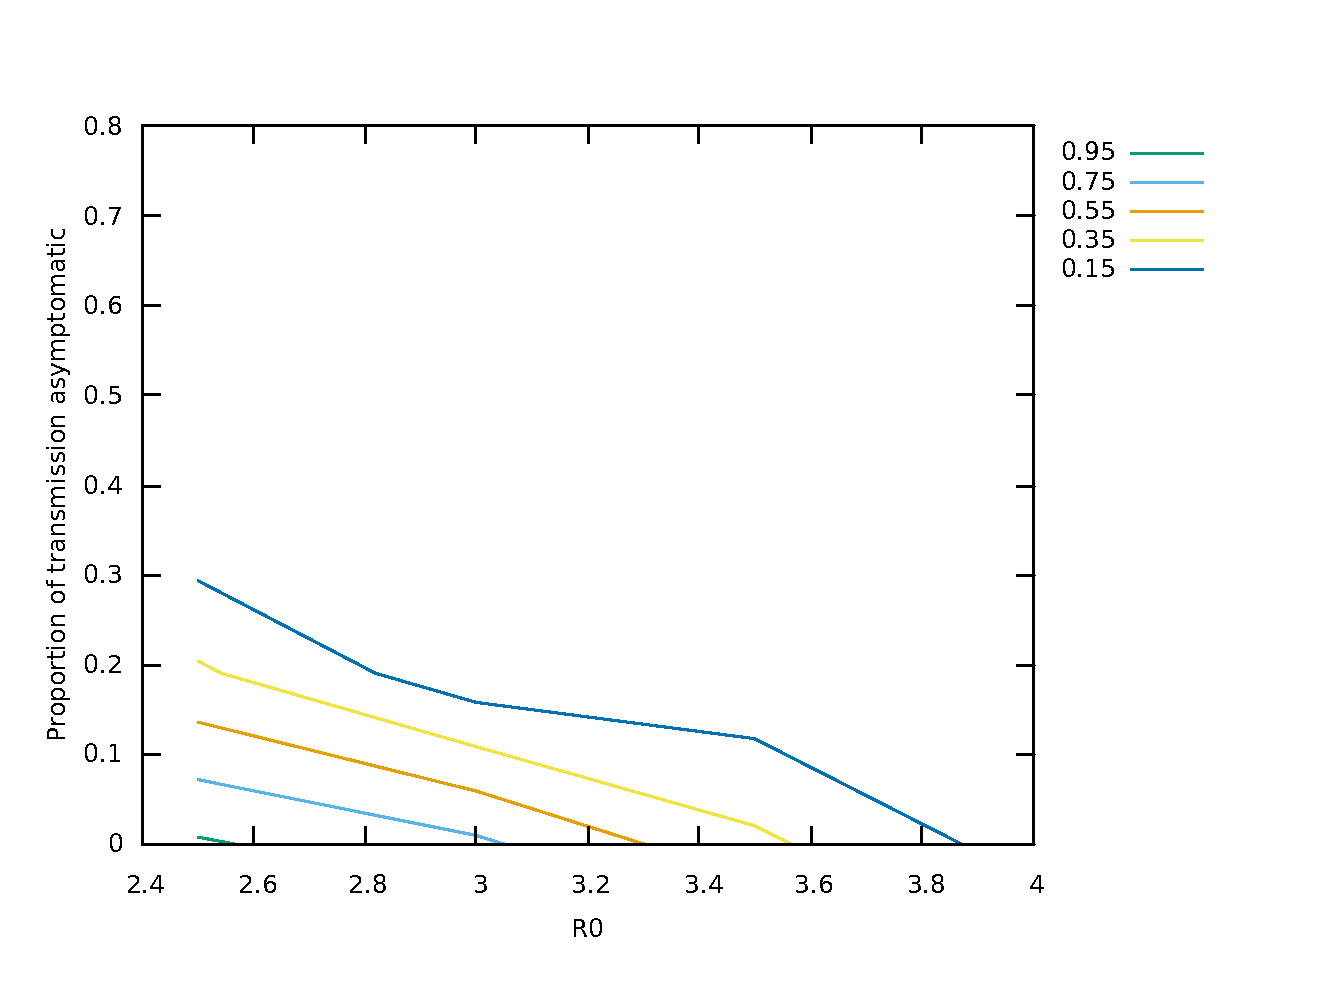
\includegraphics[width = 10cm]{baseline.pdf}
\end{center}
\caption{Probability of eradication under baseline scenario}
\label{baseline}
\end{figure}

\subsection{Workplace symptom reporting}

This scenario is the same as the baseline but with the addition that companies and schools have a duty to test an employee/student if they are seen to be symptomatic. Antigen test kits and swabs could be kept on-site and first aiders could be trained to administer the antigen test and take the swab. We assume in this scenario that a symptomatic person who elects not to self-isolate has a 90\% chance of being reported at work.

As can be seen from Figure \ref{workplaceSymptom}, this dramatically improves the probability of eradication over the baseline.

\begin{figure}
\begin{center}
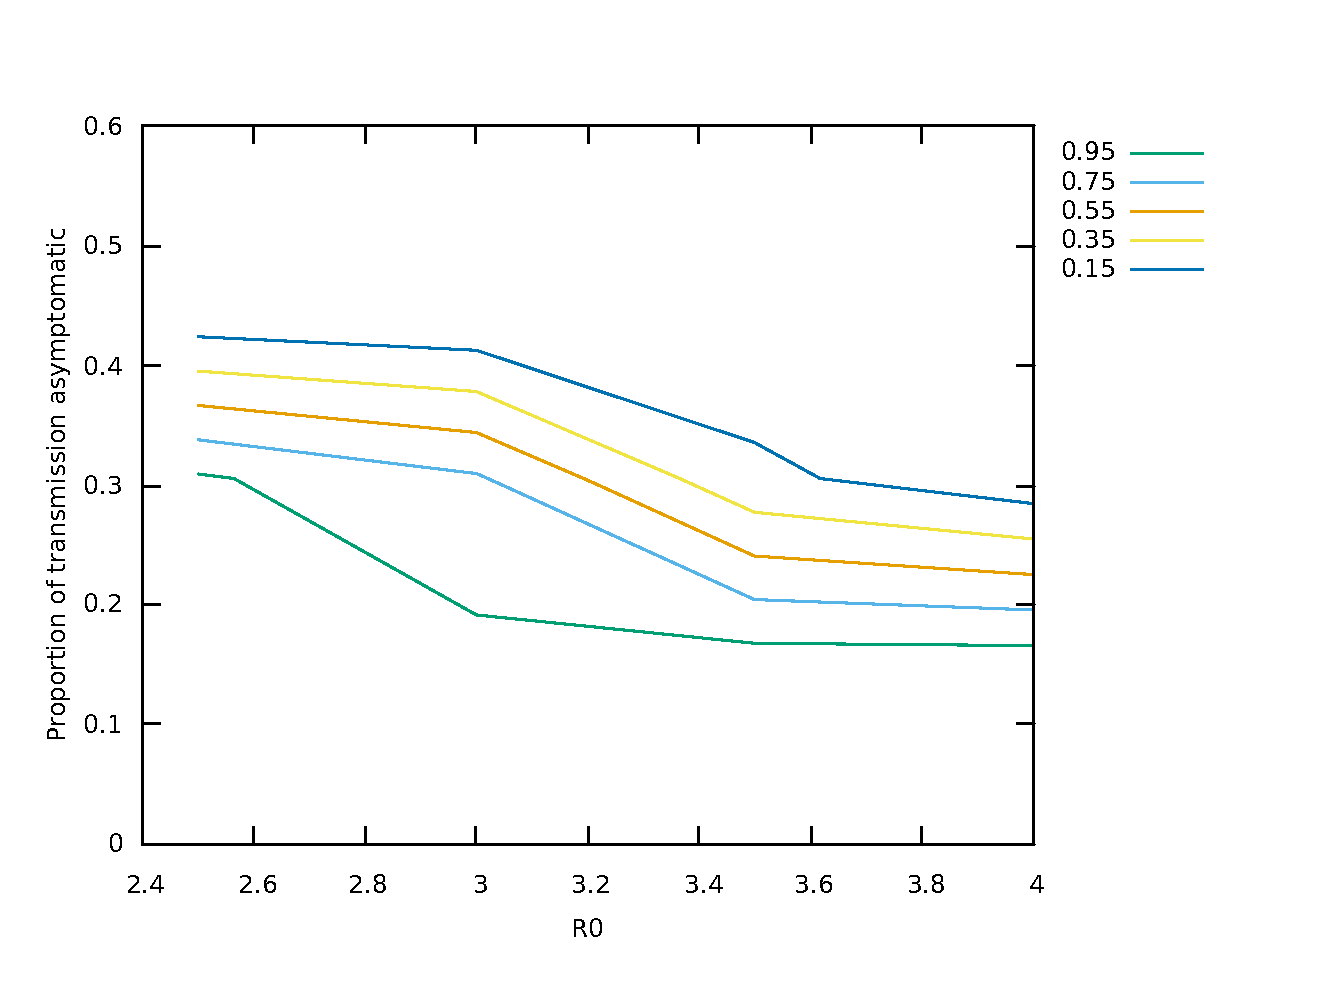
\includegraphics[width = 10cm]{workplaceSymptomMonitoring.pdf}
\end{center}
\caption{Probability of eradication under workplace symptom monitoring}
\label{workplaceSymptom}
\end{figure}

\subsection{Whole household testing}

This scenario is the same as workplace symptom reporting but with the addition that if a person tests positive, their whole household must be tested. In this case testing is mandatory rather than optional, so people who would not otherwise comply with an instruction to be tested will in this scenario be tested. See figure \ref{householdAndWorkplaceSymptom}.

\begin{figure}
\begin{center}
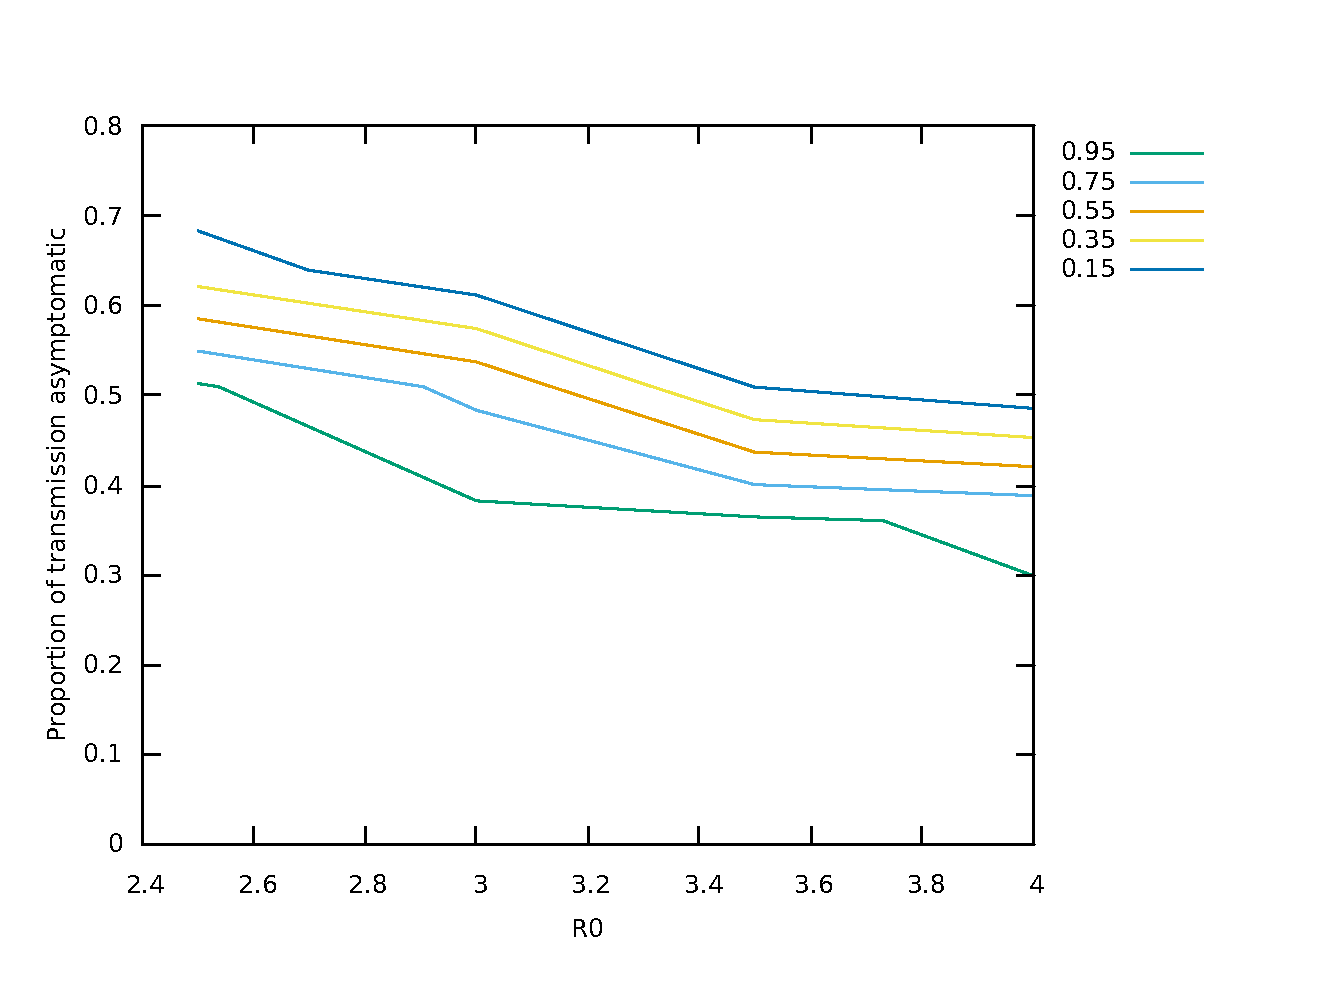
\includegraphics[width = 10cm]{householdEnforcement.pdf}
\end{center}
\caption{Probability of eradication under whole household testing and workplace symptom monitoring}
\label{householdAndWorkplaceSymptom}
\end{figure}

\subsection{Whole household testing and workplace tracing}

In this scenario, all the above measures are in place but companies and schools have an additional duty to ensure contact tracing in the workplace. This will likely consist of issuing a bluetooth device (not necessarily a smart phone) to any employee or student who doesn't already have a contact-tracing app on their phone. The device would be carried whenever the person is in the workplace. See figure \ref{householdAndWorkplaceEnforcement} for the probability of eradication under this scenario

\begin{figure}
\begin{center}
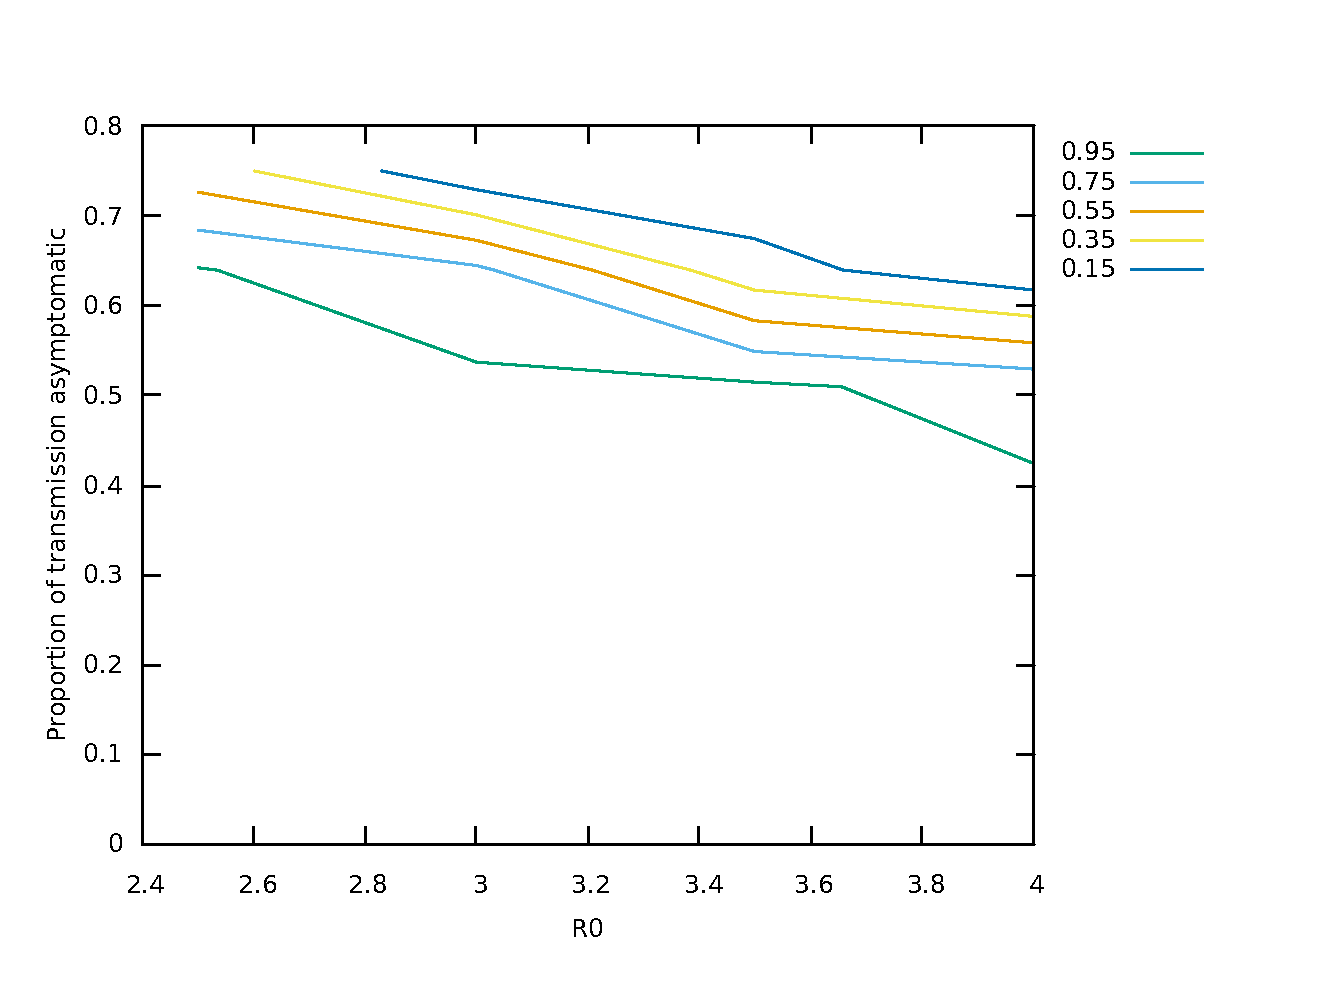
\includegraphics[width = 10cm]{workplaceAndHouseholdEnforcement.pdf}
\end{center}
\caption{Probability of eradication under whole household testing and workplace tracing}
\label{householdAndWorkplaceEnforcement}
\end{figure}

\section{Description of the Model}

The model we use is based on the stochastic branching model described in \cite{hellewellfeasibility} but implemented as an agent-based, discrete event simulation. This allowed us to implement more complex containment strategies with less effort at the cost of execution speed. It also allows us to correctly capture the tracing of infected agents via a previously untraced mutual infector, which is not properly captured in a stochastic branching model. In the presence of many asymptomatic carriers, and very fast and accurate tracing, this is expected to be important.

The model consists of infected agents, each of which belongs to a household. Once infected, an agent goes though an incubation period with duration drawn from a Weibull distribution with shape parameter $2.322737$ and scale parameter $6.492272$\cite{backer2020incubation}. The transmission generation interval (i.e. time from exposure to transmission) is drawn from a skew normal distribution with location parameter equal to the clinical onset time (i.e. end of the incubation period) and scale parameter of 2.0. In order to avoid unrealistically early transmissions, the generation interval was bounded to a minimum of 1 day. A proportion of agents are asymptomatic, these will never have clinical onset and are assumed to be $\frac{2}{3}$ as infectious as symptomatic carriers\cite{ferguson2020impact}. The number of susceptible agents that an infected agent will infect if not isolated is drawn from a negative binomial distribution with overdispersion parameter $10.0$\cite{zhuang2020preliminary}\cite{riou2020pattern} and mean of $\frac{3R_0}{3 - \rho}$ for symptomatic agents and $\frac{2R_0}{3 - \rho}$ for asymptomatic agents where $\rho$ is the probability of being asymptomatic and $R_0$ is the basic reproductive number. At each transmission event a new infected agent is created, unless the infecting agent is isolated, in which case the event has no effect. Following\cite{Ferrettieabb6936} 10\% of transmission is ``environmental'' (i.e. via surfaces, air-conditioning etc.) meaning that it cannot be traced to the infector even if they have the app installed.

Each transmission event occurs either in the household, at the workplace/school or in the community. It is assumed that 5\% of the population have immunity from a previous outbreak. After an outbreak we would expect there to be a correlation in immunity between members of the same household since during the peak, under ``stay at home'' rules, if one member of a household contracts the disease it is likely that all other members will also contract it, so we end up with immune and susceptible households. This means that only members of susceptible households can become infected during the contact-tracing stage, so we assume no household members of an infected agent are immune. The relative probability of transmission in the household is assumed to be 3 times greater in the household than in the other locations. This was calibrated in order to obtain equal aggregate numbers of transmission events in each location under no intervention\cite{ferguson2020impact}. Although studies from Korea and US suggest this factor may be higher\cite{OsongReport}\cite{burke2020active}, the uncertainty is high and we keep this at 3 for the UK due to the prevalence of HMOs in the UK. The distribution of number of members in a household was calibrated against\cite{smithHouseholds}.

The source code of the model is available at \href{https://github.com/danftang/Covid19}{https://github.com/danftang/Covid19}

\section{Discussion}

We have suggested a number of increasingly effective, but also increasingly draconian measures that could be used to improve the chances that contact tracing is successful in avoiding another resurgence of COVID-19. It is envisaged that the measures would be implemented in response to the evolving situation and only when absolutely necessary to avoid a resurgence. With all these measures in place, containment is likely, but if $R0$ and total asymptomatic transmission turns out to be very high further measures may be necessary. In this case, social distancing and public hygiene measures would need to be implemented in addition. Although some of the measures discussed here may seem authoritarian, they must be put in the context of the situation we face. Life with contact tracing will be very close to normal for the vast majority of the population and will be much less socially disruptive, and will impinge much less on personal freedoms, than a national lock-down.

%\bibliographystyle{unsrtnat}
\bibliographystyle{unsrturl}
%\bibliographystyle{alpha}
%\bibliographystyle{plainurl}
%\bibliographystyle{apalike} 
%\bibliographystyle{apacite}
\bibliography{references}

\end{document}
